%======================================================================
\chapter{System Architecture}
\label{ch: Chapter2}
%======================================================================

%----------------------------------------------------------------------
\section{System Block Diagram}
%----------------------------------------------------------------------
The overall system architecture of this project consists of two subsystems which
are the Mobile Cart and the Remote Target, which is held by the user or
customer, as shown in Fig. \ref{fig:sys_block_diag}. The proposed smart robotic
cart is a wheeled robot that sends and receives radio signals to follow the
remote target which acts as the beacon for the robotic cart system.

\vspace*{12pt}
\noindent
The high-level system block diagram of the proposed robotic cart (prototype) is shown in Fig. \ref{fig:sys_block_diag}. There are three inputs to the proposed cart system. The robotic cart is supplied with power through a battery that is mounted in the chassis of the robotic cart. There will be an on/off switch to allow the system to be powered down when not in use. This will save the battery from being drained by the XBees in the reflector array. The motion of the robotic cart is dependent on the motion of the remote.

\begin{figure}[H]
  \centering
  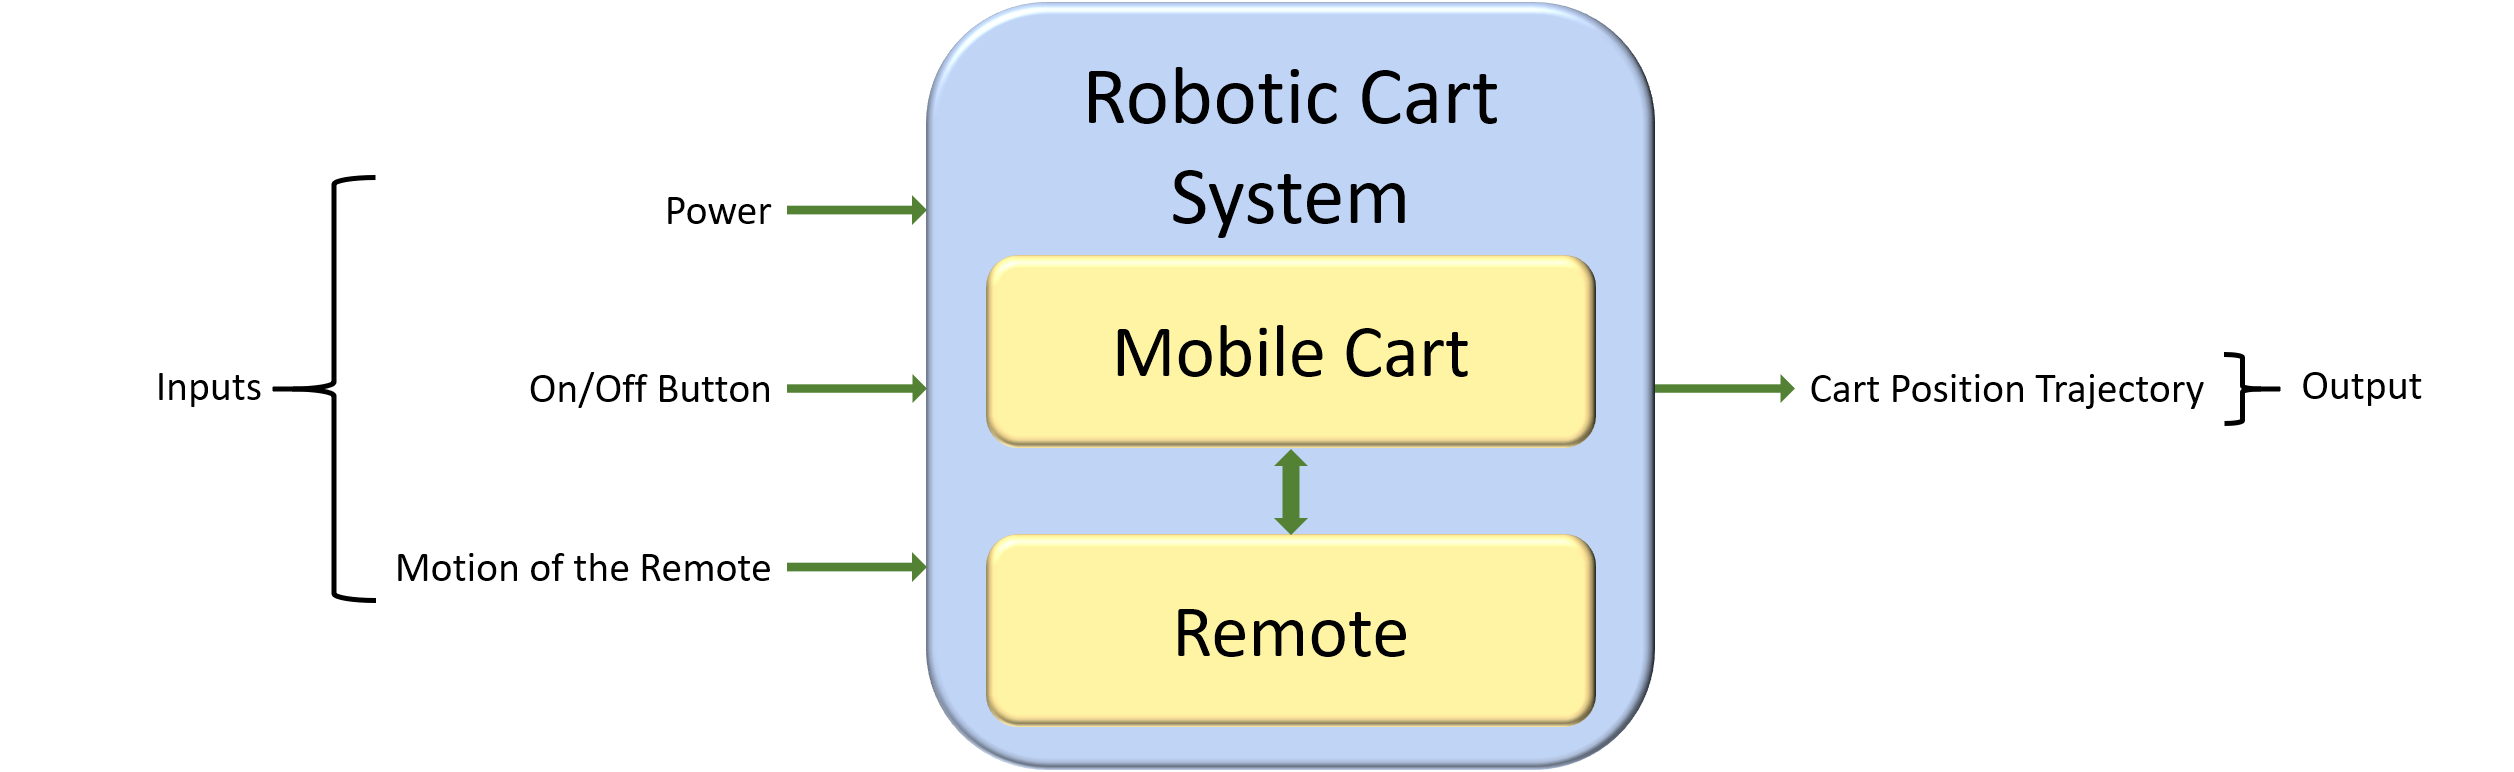
\includegraphics[width=\textwidth]{figs/img/systemBlockDiagram.png}
  \caption{System level block diagram detailing inputs and outputs to the
    robotic cart system.}
	\label{fig:sys_block_diag}
\end{figure}

\vspace*{12pt}
\noindent
The main output of the system is the position trajectory of the robotic cart in its environment. When the user moves with the remote target, the robotic cart is designed to follow the user.



%----------------------------------------------------------------------
\section{Subsystem Block Diagrams}
%----------------------------------------------------------------------
The Mobile Cart and the Remote Target subsystems are two separate operations
within the robotic cart system that run simultaneously. The two subsystems
communicate with one another by relaying radio messages between them. The first
block diagram is of the Remote Target subsystem shown in Fig.
\ref{fig:remote_block_diag}. Of the two subsystems the Remote Target is the
simplest since it only requires an XBee module attached to a 7.4V Li-Po battery
with a voltage regulation circuit since the XBee has a smaller input voltage of
3.3 volts. The two inputs for this system are the battery power and the incoming
RF messages which are passed through the RF transceiver Module and output the
outgoing RF messages.

\begin{figure}[H]
  \centering
  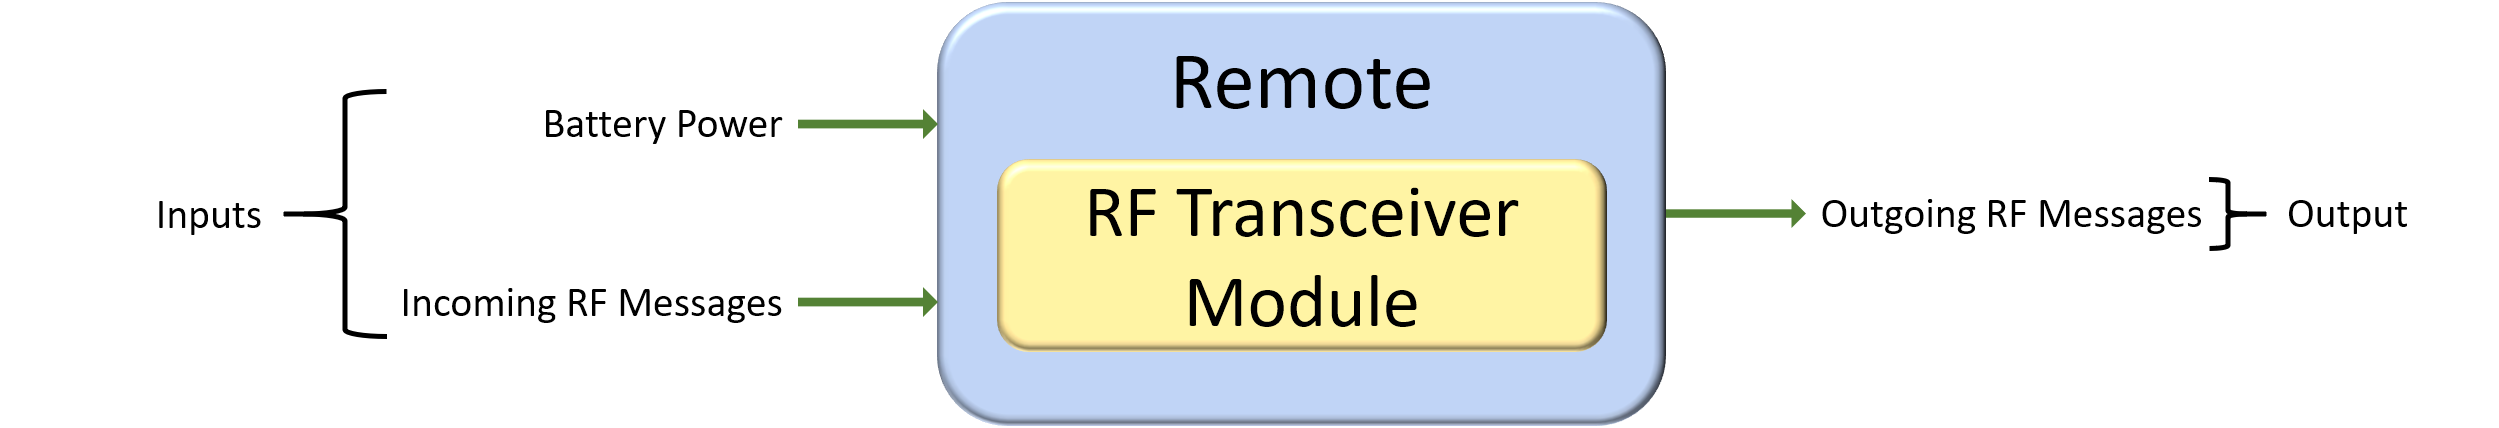
\includegraphics[width=\textwidth]{figs/img/remoteBlockDiagram.png}
  \caption{Remote Target block diagram}
  \label{fig:remote_block_diag}
\end{figure}

\vspace*{12pt}
\noindent
The Mobile Cart subsystem block diagram, shown in Fig.
\ref{fig:mobile_block_diag}, is the most complex of the two subsystems.The cart requires a power source, which will be a 7.4V, 8,000 mAh Li-Po battery since the
Li-Po works well with powering the embedded computer (BeagleBone Blue). The
power to the subsystem will be toggled by an on/off switch located on the
chassis of the robotic cart. The final input to the mobile cart subsystem is the
incoming RF signals. These incoming RF signals are passed to the direction
sensitive RF receivers which output the signals to the dual-direction
multiplexer. The dual-direction multiplexer then takes the four inputs from the
direction sensitive RF receivers and passes one output into the embedded
computer. Once the embedded computer gets these signals it can calculate the
localization and navigation algorithms and pass the information to the DC
motors.

\begin{figure}[H]
  \centering
  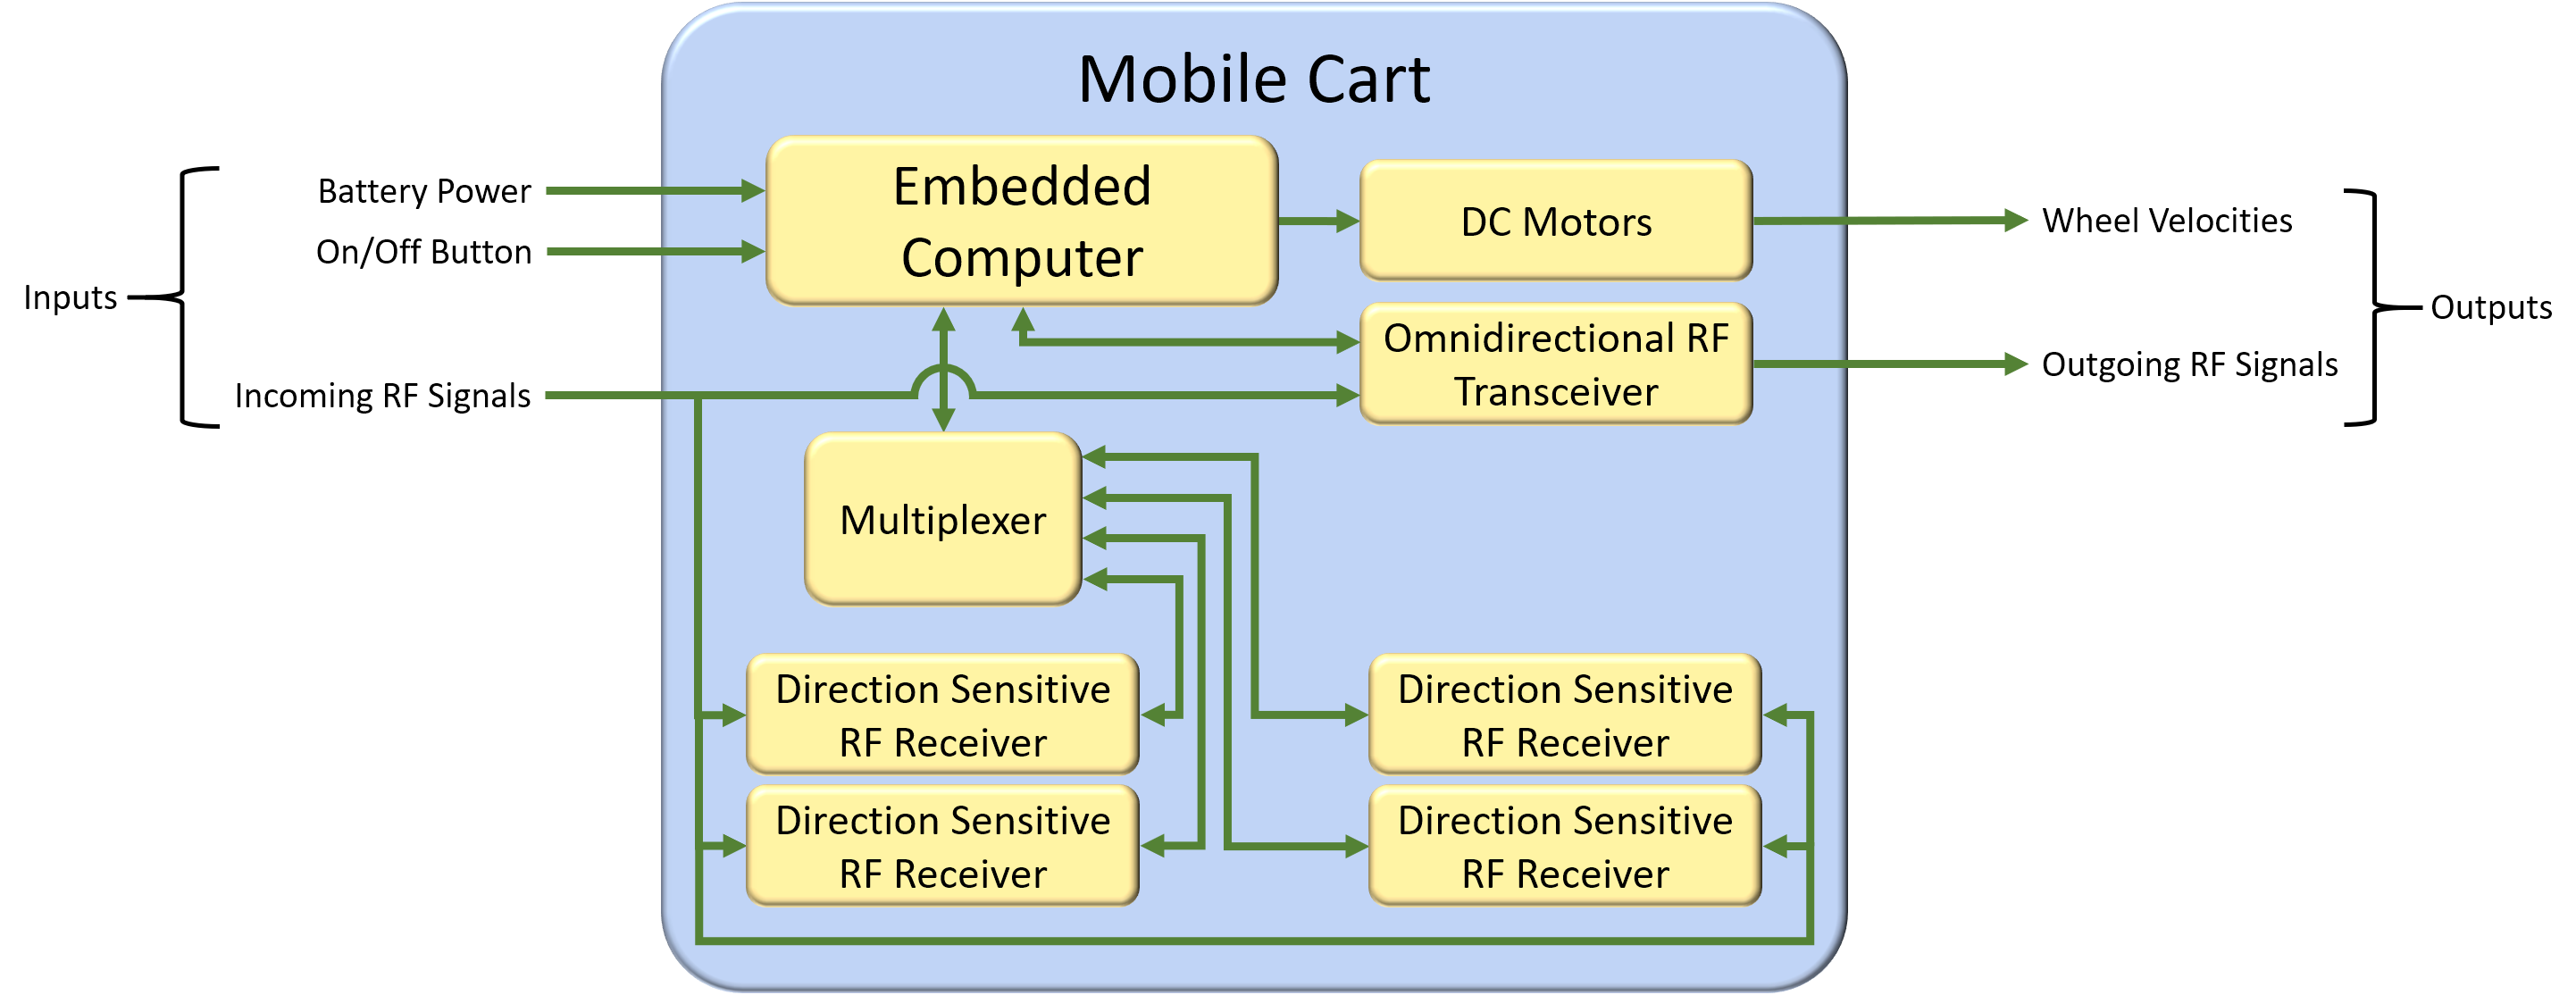
\includegraphics[width=\textwidth]{figs/img/mobileCartBlockDiagram.png}
  \caption{Block diagram showing the subsystem-level components of the proposed robotic cart.}
  \label{fig:mobile_block_diag}
\end{figure}

\vspace*{12pt}
\noindent
There are two outputs of the mobile cart subsystem. The first is the wheel velocities that move the cart and are passed from the DC motors. Lastly, the incoming RF signals are passed to our omnidirectional RF transceiver which outputs the outgoing RF signals.


%----------------------------------------------------------------------
\section{System Components}
\label{sec:System Components}
%----------------------------------------------------------------------

There are several components that are required for the mobile cart system.
Although some of these parts are available in the Bradley University laboratory,
other parts must be purchased. The parts that exist in the lab are listed in
\autoref{tab:Partslablist}. Also, \autoref{tab:Partslist} shows the list of
parts that were purchased. The parts compiled in the lists are the required
parts needed to build two smart robotic cart systems.

\begin{table}[H]
  \centering
  \caption{Parts Available in Laboratory}
  \begin{tabular}{c|c}
      \toprule
      \textbf{Quantity} & \textbf{Parts}\\
      \toprule
      2 & Budget Bot Chassis\\
      4 & 10 uF Ceramic Capacitor\\
      4 & LM1117 Regulator\\
      8 & 9V Batteries\\
      4 & Solderable PCB Boards\\
      3 & XBee USB Adapter\\
      \bottomrule
      %\multicolumn{2}{r|}{\textbf{Total}} & \$ 562.34\\
      %\bottomrule
  \end{tabular}
  %\caption{Parts Available in Laboratory}
  \label{tab:Partslablist}
\end{table}

\begin{table}[H]
  \centering
  \caption{Purchased parts for the Robotic Cart Project}
  \begin{tabular}{c|c|c}
    \toprule
    \textbf{Quantity} & \textbf{Parts} & \textbf{Price}\\
    \toprule
    4 & Pololu 37D Metal Gear motor 4751 & \$ 39.95\\
    12 & XBee S2C Module & \$ 23.10\\
    10 & XBee Adapter Board & \$ 4.99\\
    2 & Twotrees 4 Lead Nema 17 Stepper Motor & \$ 9.99\\
    1 & 4-Pin JST SH Connector - 20 Pack & \$ 7.99\\
    1 & 6-Pin JST SH Connector - 10 Pack & \$ 9.99\\
    1 & Aluminum Foil Tape - 2 in x 5 yd & \$ 6.05\\
    2 & Ovonic 7.4V 8000mAh LiPo Battery & \$ 40.99\\
    4 & Multiplexers & \$ 15.99\\
    \bottomrule
    \multicolumn{2}{r|}{\textbf{Total}} & \$ 562.34\\
    \bottomrule
  \end{tabular}
  %\caption{Purchased parts for the Robotic Cart Project}
  \label{tab:Partslist}
\end{table}

\vspace*{6pt}
\noindent
The main components for this project are the Budget Bot Chassis (Fig.
\ref{fig:budgetBotChassis}), the BeagleBone Blue embedded computer (Fig.
\ref{fig:beagleboneBlue}), and the XBee S2C Modules (Fig. \ref{fig:XBeeModule}).
Another major component is the reflector array that will be used to
directionally receive the RF signals from the remote target that is with the
user.

\begin{figure}[H]
  \centering
  \begin{subfigure}[t]{0.32\textwidth}
    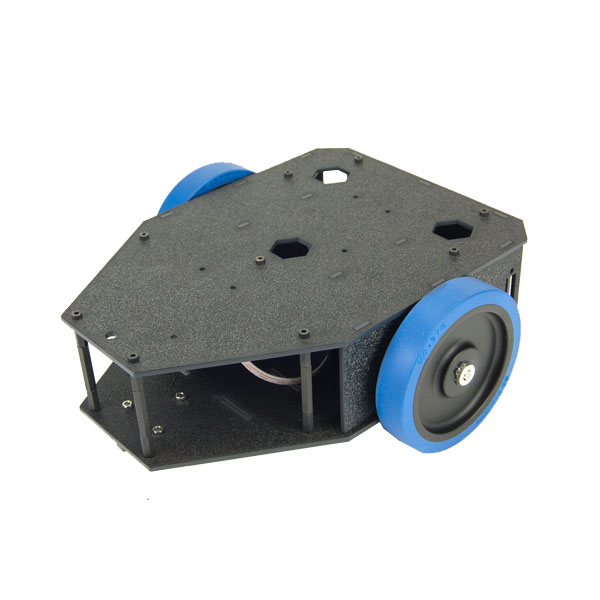
\includegraphics[width=1\textwidth]{figs/img/budgetbot_chassis}
    \captionsetup{width=\textwidth}
    \caption{Budget Bot Chassis}
    \label{fig:budgetBotChassis}
  \end{subfigure}
  \begin{subfigure}[t]{0.32\textwidth}
    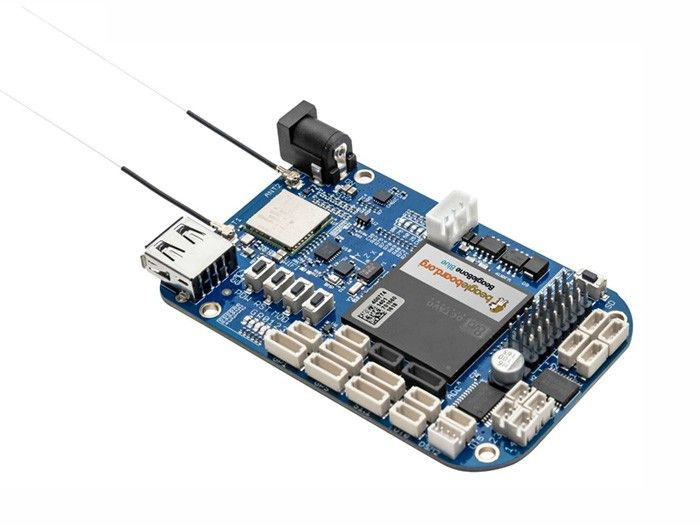
\includegraphics[width=1\textwidth]{figs/img/beaglebone_blue}
    \captionsetup{width=\textwidth}
    \caption{BeagleBone Blue}
    \label{fig:beagleboneBlue}
  \end{subfigure}
  \begin{subfigure}[t]{0.32\textwidth}
    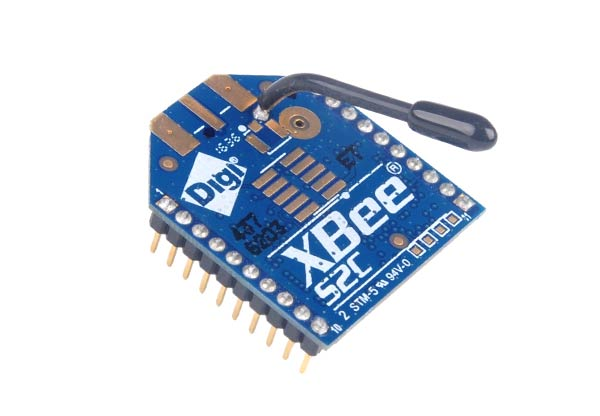
\includegraphics[width=1\textwidth]{figs/img/Xbee-S2C-Module}
    \captionsetup{width=\textwidth}
    \caption{XBee S2C Module}
    \label{fig:XBeeModule}
  \end{subfigure}
\end{figure}

\vspace*{12pt}
\noindent
The reflector array will be mounted on top of the cart with a stepper motor.
There are two reflector designs that were evaluated in this project. The first,
shown in Fig. \ref{fig:parabolodialReflector}, is a paraboloidal reflector which
maximizes the signal strength of the signals that come into the reflector
perpendicularly. Since the remote will be carried by the user, it is likely that
it will be positioned at a higher altitude than the reflector array. The
paraboloidal reflector design may not be able to pick up the signals from the
remote as well because of this. %
%
%
\begin{figure}[H]
  \centering
  \begin{subfigure}[t]{0.5\textwidth}
    \centering
    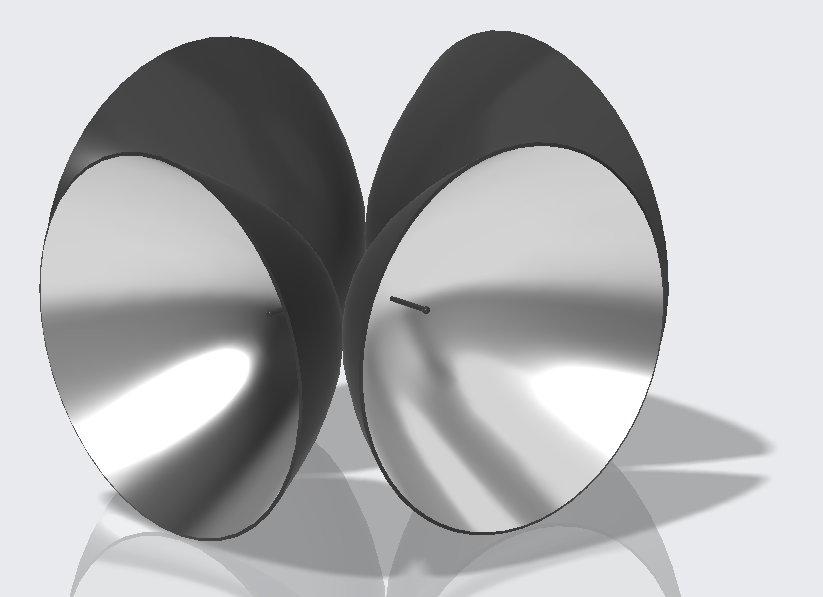
\includegraphics[height=2in]{figs/img/paraboloidalReflector}
    \captionsetup{width=\textwidth, justification=raggedright}
    \caption{Paraboloidal Reflector Model}
    \label{fig:parabolodialReflector}
  \end{subfigure}
  \begin{subfigure}[t]{0.4\textwidth}
    \centering
    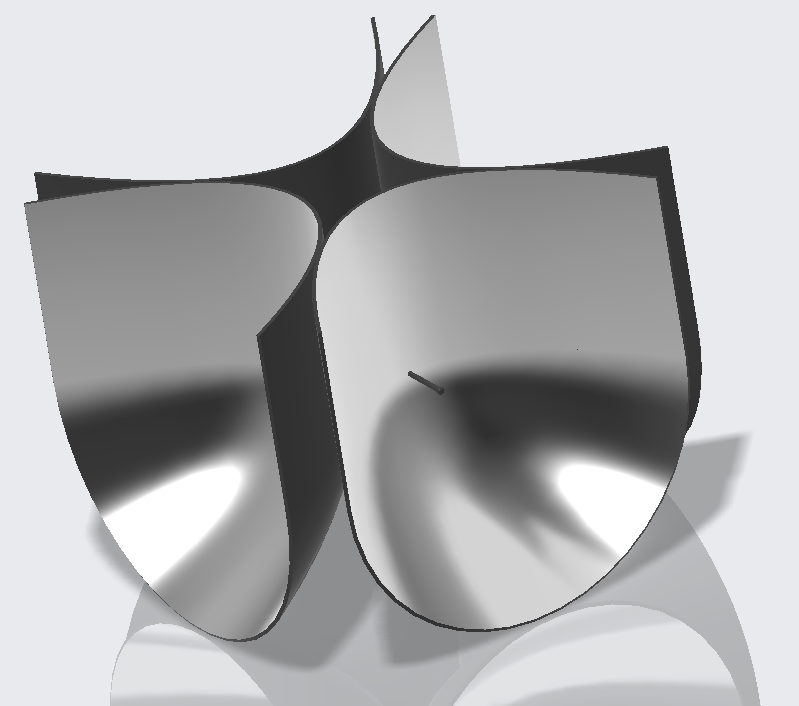
\includegraphics[height=2in]{figs/img/parabolicReflector}
    \captionsetup{width=\textwidth, justification=raggedright}
    \caption{Combined Parabolic/Paraboloidal Reflector}
    \label{fig:parabolicReflector1}
  \end{subfigure}
\end{figure}
%
To solve this problem, a combination parabolic/paraboloidal reflector was
designed, as shown in Fig. \ref{fig:parabolicReflector1}. The lower half of this
reflector is paraboloidal in shape to limit the signals coming from below. The
upper part of the reflector is strictly parabolic. This shape focuses the
signals in the horizontal plane, but allows signals from above to still be
received. The plan is to construct both of these reflector designs by 3D
printing the frames, then lining them with reflective foil tape. Both models
will then be tested to determine which design works better.


%----------------------------------------------------------------------
\section{Operation of Robotic Cart System}
\label{sec:Operation of Robotic Cart System}
%----------------------------------------------------------------------
The mobile cart was controlled by a central embedded computer which is the BeagleBone Blue since it is ideal in robotics control. Two DC motors were used to drive wheels and move the cart. Five XBee modules on the cart were used to allow communication with the remote target. One of these radio sensors was mounted on top of the cart to broadcast in all directions. The other four sensors were placed inside parabolic reflectors at right angles to each other. This sensor array was mounted on a stepper motor to allow rotation.


%%% Local Variables:
%%% mode: latex
%%% TeX-master: "../finalReport"
%%% End:
